
%(BEGIN_QUESTION)
% Copyright 2015, Tony R. Kuphaldt, released under the Creative Commons Attribution License (v 1.0)
% This means you may do almost anything with this work of mine, so long as you give me proper credit

\noindent

\vskip 5pt

\vskip 5pt
\begin{center}
\textbf{Styresystemer -- Nivå 1 }
\vskip 5pt 
\textbf{Arbidsoppdrag på Stasjon 11}
\vskip 5pt 
\textbf{Oppsett av målesystemer for temperatur}
\end{center}

\textbf{Introdusjon}

\vskip 5pt 
I dette oppdraget skal du sette opp og kalibrere to målesystemer for temperatur. Det ene systemet skal benytte en transmitter fra GM (D1072S) og det andre en fra Pepperl+Fuchs (KFD2-UT2-Ex1). Begge disse transmitterne er laget for bruk i EX områder det skal vi ikke bry oss med i dette oppsraget. 
\\
Begge målesystemene må settes opp med software fra leverandøren:
\\
\textbf{Pepperl+Fuchs}
\\
For å programmere KFD2-UT2-Ex1, trenger du adapteren K-ADP-USB, samt programmet Pactware og Tilhørende DTM.
\\

Programvaren laster du ned gratis hos oss:
\\
\href {https://www.pepperl-fuchs.com/norway/no/classid_163.htm?view=productdetails&prodid=83574#software}{PACTware 5.X}
\\
\href {https://www.pepperl-fuchs.com/norway/no/classid_1804.htm?view=productdetails&prodid=32802}{DTM Interface Technology}
\\
 

\href{https://files.pepperl-fuchs.com/webcat/navi/productInfo/doct/tdoct1599c_eng.pdf?v=20200320004907}{Veiledning} Installation and configuration guide Device Type Manager (DTM)
\\  
Eventuellt trenger du kanskje denne, men prøv først uten:
\\
\href {https://www.pepperl-fuchs.com/norway/no/classid_1805.htm?view=productdetails&prodid=27434}{Microsoft .NET}


\vskip 5pt 

\textbf{GMI}
\\
Software til GMI D1072s finner du i mappen software vi bruker og verktøy (SWC1090.exe)
\\
Målesystemene skal ha følgende måleområder:
\begin{itemize}[noitemsep]
\item GMI 10-40°C
\item Pepperl+Fuchs -5-100°C
\end{itemize}

\vskip 5pt 

Det må fylles ut kalibreringssertifikat for begge målesystemene. 


$$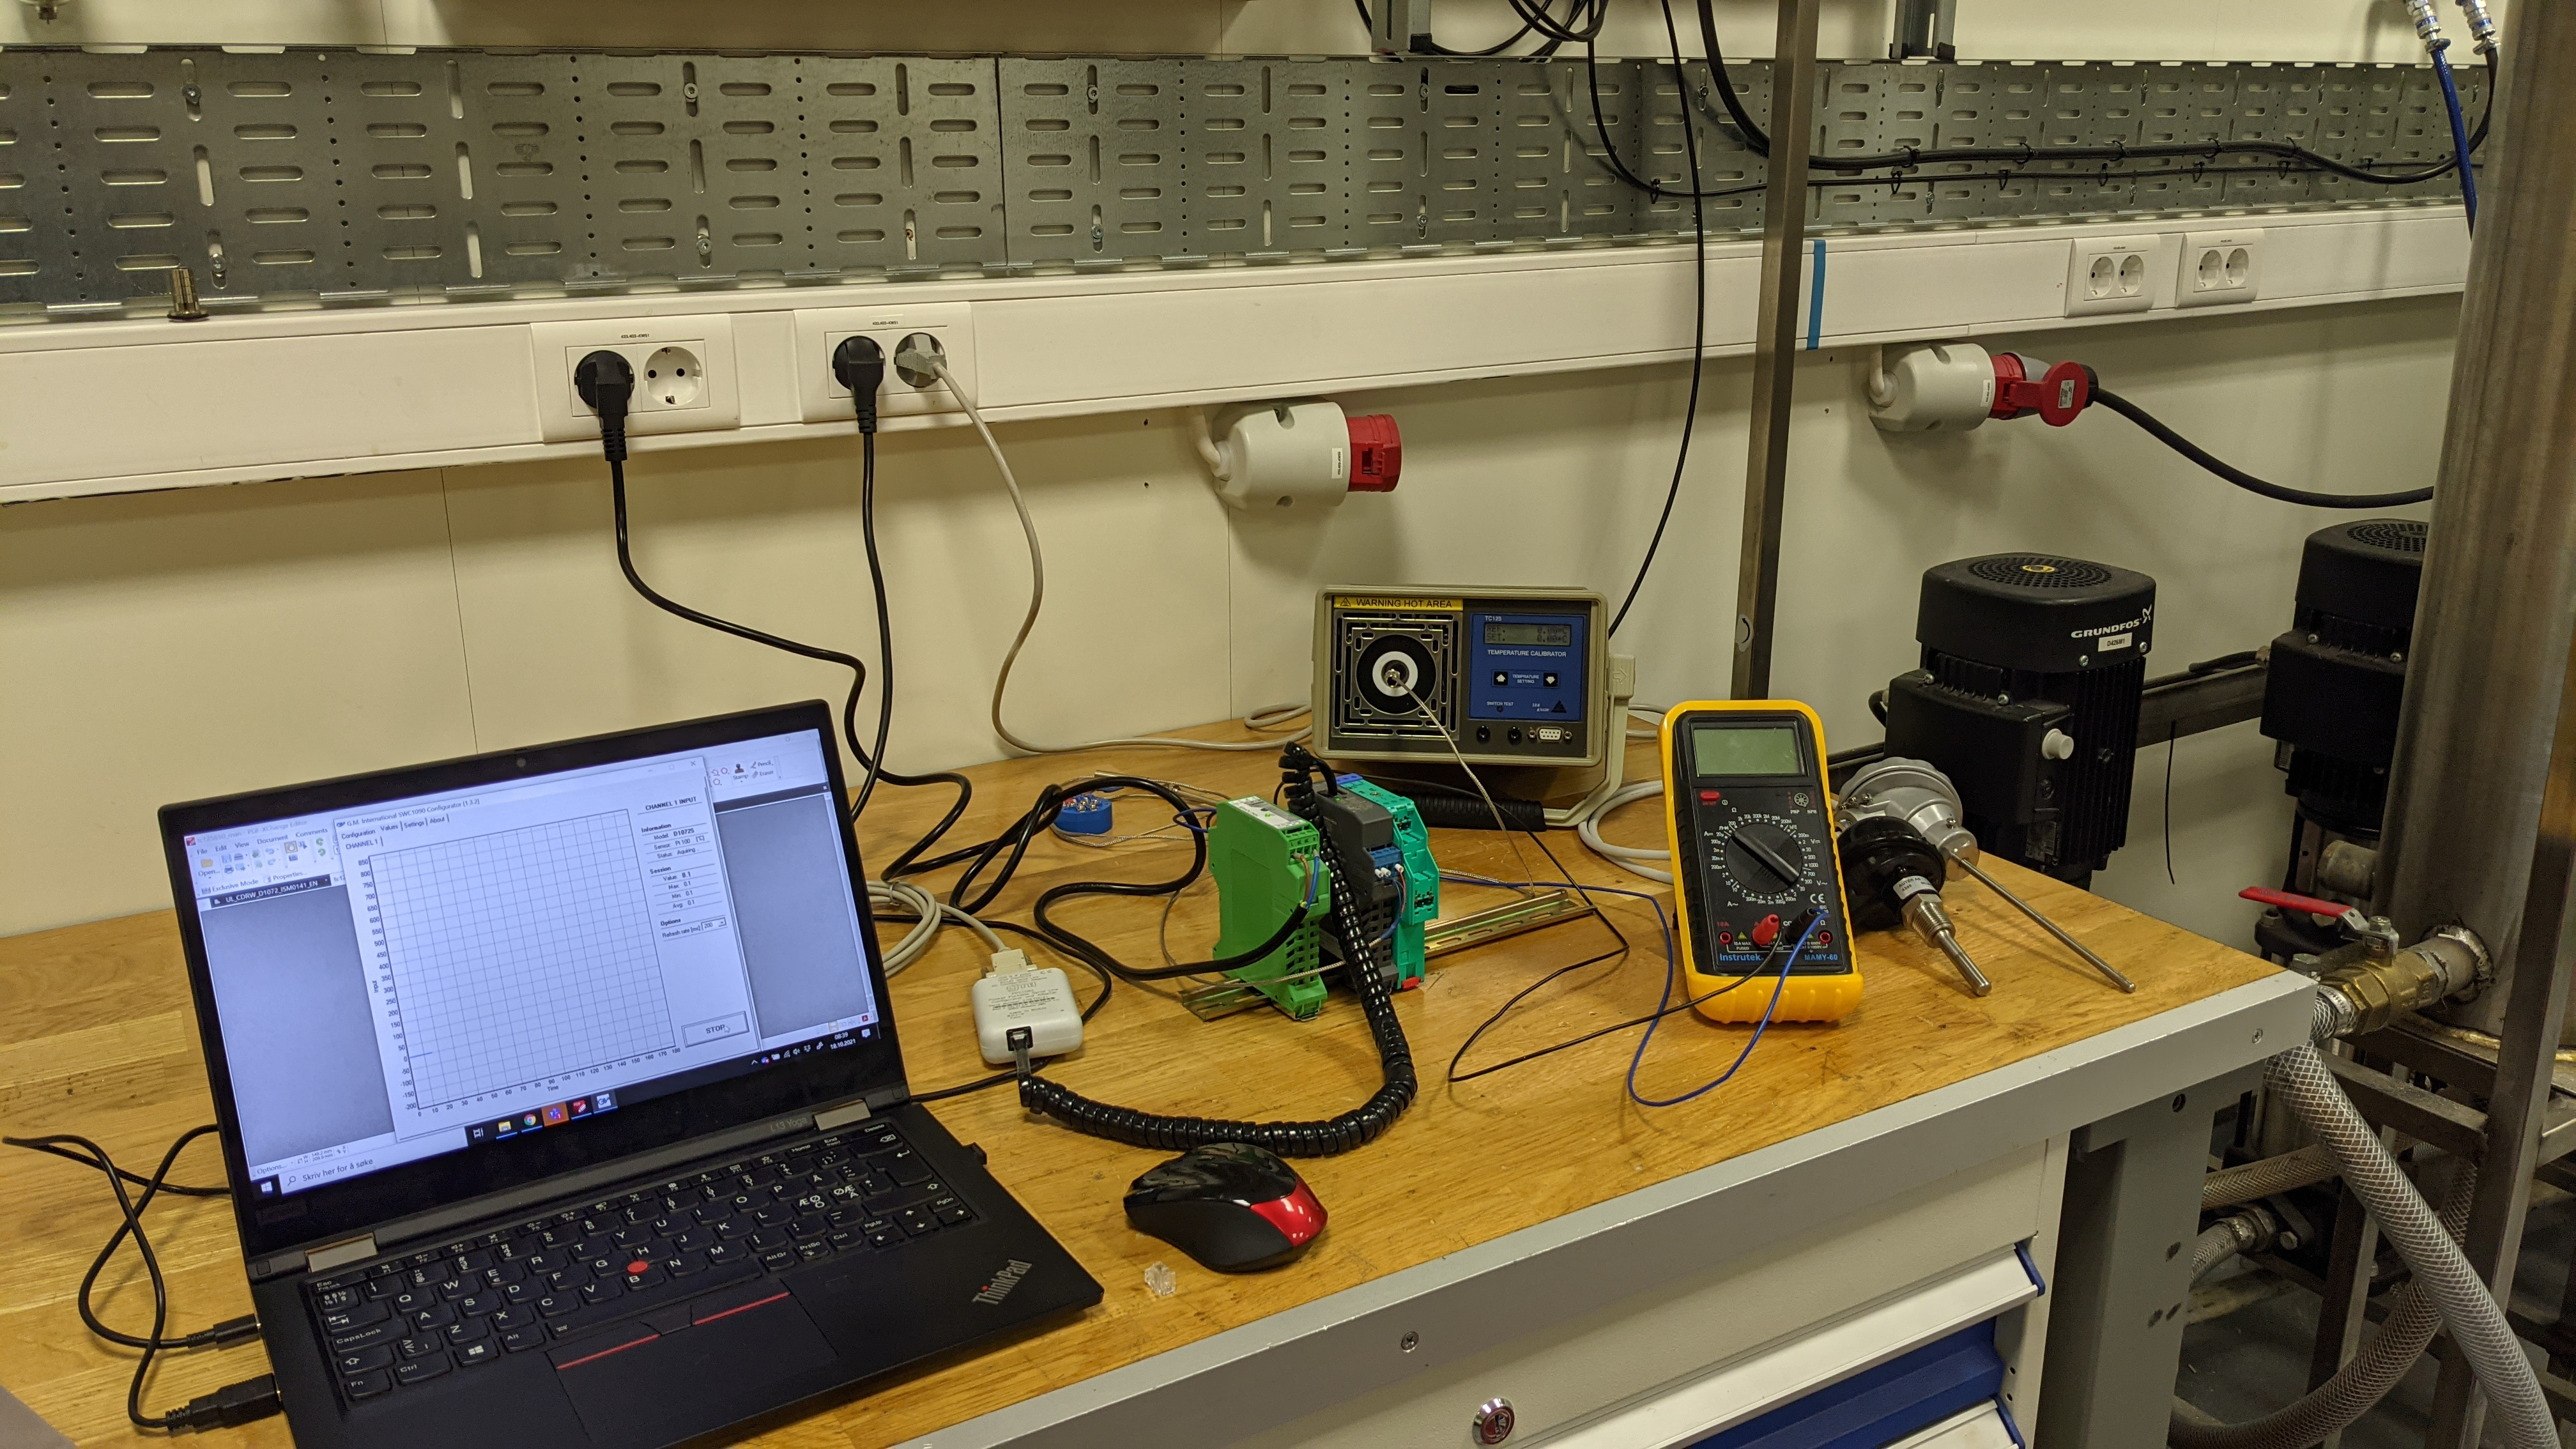
\includegraphics[width=13cm]{i04841x01.jpg}$$\\
\textbf{Arbidsoppdrag -- teorioppgaver}

\vskip 5pt 
\href {https://autofaget.no/temp/node2.html}{Leseoppgave}

\vskip 5pt 
\textbf{Arbidsoppdrag -- planlegging}

\textbf{Arbidsoppdrag -- gjennomføring}

\textbf{Arbidsoppdrag -- dokumentasjon}








\underbar{file i04841}
\vfil \eject
%(END_QUESTION)





%(BEGIN_ANSWER)


%(END_ANSWER)





%(BEGIN_NOTES)


%INDEX% Arbeisdoppdrag, Kompetanse, Nivå 1, Stasjonxx, Mal

%(END_NOTES)


